\documentclass{beamer}
\usetheme{Rochester}
\usecolortheme{seahorse}
\usepackage{amsmath}
\usepackage{tikz}
\usepackage{graphicx}
\usepackage{caption}
\usepackage{colortbl} % Needed for \columncolor and \rowcolor

\definecolor{myPurple}{RGB}{150, 0, 150} % Define a custom purple color
\definecolor{myLightBlue}{rgb}{0.82, 0.92, 1.00}
\definecolor{myGray}{rgb}{0.85, 0.85, 0.85}
\definecolor{seahorsePurple}{RGB}{214, 214, 240}

\setbeamertemplate{itemize item}{\color{myPurple}\textbullet} % Change bullet color and shape
\setbeamertemplate{itemize subitem}{\color{myPurple}\textbullet} % Change subitem as well
\setbeamertemplate{itemize subsubitem}{\color{myPurple}\textbullet} % Change subsubitem as well

\title{Search within a collection of documents}
\subtitle{Mathematical Modelling}
\author{Nik Jenič, Tian Ključanin, Maša Uhan}
\date{}

\begin{document}

\frame{\titlepage}

\begin{frame}{Problem Introduction}
    \begin{itemize}
        \item Finding relevant documents according to our search
    \end{itemize}
\end{frame}

\begin{frame}{Solution}
    \begin{itemize}
        \item LSI - Latent Semantic Indexing
    \end{itemize}
    \begin{figure}
        \centering
        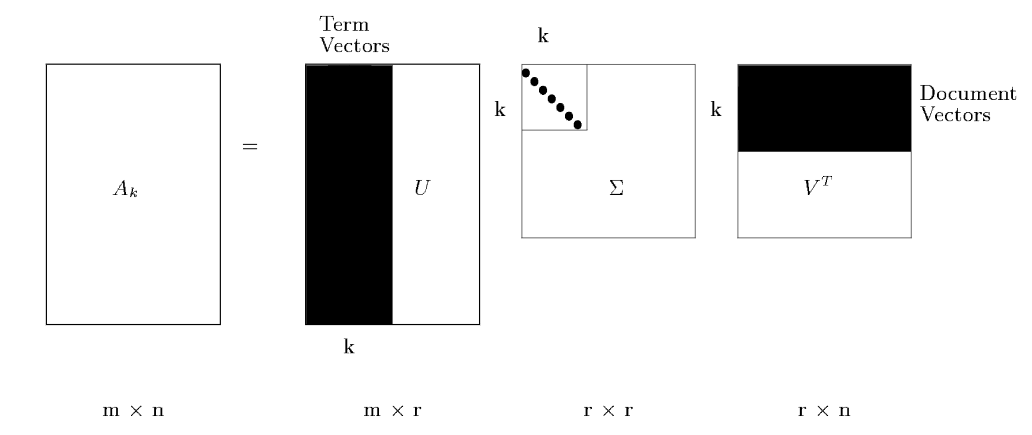
\includegraphics[width=0.9\textwidth]{../Slike/svd.png}
        \caption{Mathematical representation of $A_k$}
        \label{fig:matrixA}
      \end{figure}
\end{frame}

\begin{frame}{Optimization}
    \begin{itemize}
        \item Giving words different weights
        \item Different ways of calculating the weights
    \end{itemize}
    \begin{center}
        \[
            a_{ij} = L_{ij} \cdot G_i
        \]
        \[
            L_{ij} = \log (1 + f_{ij}), \quad G_i = 1 - \sum_{j} \frac{p_{ij} \log (p_{ij})}{\log n}, \quad p_{ij} = \frac{f_{ij}}{g_{f_i}}
        \]
    \end{center}
\end{frame}

\begin{frame}{Additional Improvements to the Solution}
    \begin{itemize}
        \item Adding new documents without recalculation of SVD
        \item Adding new words without recalculation of SVD
    \end{itemize}
\end{frame}

\begin{frame}{Results}
    \begin{itemize}
        \item Unoptimized Solution:
    \end{itemize}
    \centering % This centers the table on the slide
    \resizebox{\textwidth}{!}{%
        \begin{tabular}{|c|c|c|c|c|c|c|c|c|c|}
        \hline
        \rowcolor{seahorsePurple}
        & \textbf{0.10} & \textbf{0.20} & \textbf{0.30} & \textbf{0.40} & \textbf{0.50} & \textbf{0.60} & \textbf{0.70} & \textbf{0.80} & \textbf{0.90} \\ \hline
        \cellcolor{seahorsePurple}k=\textbf{10}   & 642.0 & 620.0 & 583.8 & 539.1 & 478.3 & 394.5 & 294.7 & 163.4 & 55.38 \\ \hline
        \cellcolor{seahorsePurple}k=\textbf{50}    & 395.5 & 349.9 & 282.6 & 221.0 & 170.1 & 116.9 & 93.88 & 73.63 & 30    \\ \hline
        \cellcolor{seahorsePurple}k=\textbf{100}   & 436.0 & 397.2 & 322.9 & 251.9 & 185.2 & 122.6 & 100.7 & 70    & 22    \\ \hline
        \cellcolor{seahorsePurple}k=\textbf{250}   & 545.4 & 513.8 & 451.6 & 360.4 & 257.2 & 193.3 & 127.7 & 83    & 26    \\ \hline
        \cellcolor{seahorsePurple}k=\textbf{500}   & 649.4 & 626.7 & 571.4 & 471.2 & 354.9 & 240.6 & 156   & 79    & 22    \\ \hline
        \cellcolor{seahorsePurple}k=\textbf{750}   & 649.4 & 626.7 & 571.4 & 471.2 & 354.9 & 240.6 & 156   & 79    & 22    \\ \hline
        \cellcolor{seahorsePurple}k=\textbf{1000}  & 649.4 & 626.7 & 571.4 & 471.2 & 354.9 & 240.6 & 156   & 79    & 22    \\ \hline
        \end{tabular}
    }
\end{frame}

\begin{frame}{Results}
    \begin{itemize}
        \item Optimized Solution:
    \end{itemize}
    \centering % This centers the table on the slide
    \resizebox{\textwidth}{!}{%
        \begin{tabular}{|c|c|c|c|c|c|c|c|c|c|}
        \hline
        \rowcolor{seahorsePurple}
        & \textbf{0.10} & \textbf{0.20} & \textbf{0.30} & \textbf{0.40} & \textbf{0.50} & \textbf{0.60} & \textbf{0.70} & \textbf{0.80} & \textbf{0.90} \\ \hline
        \cellcolor{seahorsePurple}k=\textbf{10}   & 71.18 & 71.18 & 71.18 & 71.18 & 70.72 & 68.47 & 68.47 & 63.06 & 44.12 \\ \hline
        \cellcolor{seahorsePurple}k=\textbf{50}    & 300.6 & 300.6 & 300.0 & 298.9 & 286.6 & 259.3 & 198.7 & 128.5 & 57.95 \\ \hline
        \cellcolor{seahorsePurple}k=\textbf{100}   & 442.1 & 442.1 & 441.2 & 417.0 & 354.4 & 273.8 & 180.7 & 116.5 & 58 \\ \hline
        \cellcolor{seahorsePurple}k=\textbf{250}   & 637.2 & 636.5 & 622.4 & 547.8 & 426.8 & 304.0 & 213.5 & 128.8 & 61 \\ \hline
        \cellcolor{seahorsePurple}k=\textbf{500}   & 726.5 & 722.5 & 674.8 & 576.7 & 435.6 & 325.3 & 201.0 & 102 & 65 \\ \hline
        \cellcolor{seahorsePurple}k=\textbf{750}   & 753.3 & 741.5 & 685.0 & 589.2 & 459.6 & 322.3 & 219 & 123 & 56 \\ \hline
        \cellcolor{seahorsePurple}k=\textbf{1000}  & 673.5 & 657.3 & 604.0 & 499.4 & 409.7 & 316.6 & 232 & 141 & 70 \\ \hline
        \end{tabular}
    }
\end{frame}




\begin{frame}{Discussion}
    \begin{itemize}
        \item NE PUSTIT PRAZNO
    \end{itemize}
\end{frame}

\begin{frame}{References}
    \begin{itemize}
        \item Source for Figure~\ref{fig:matrixA}: M. W. Berry, S.T. Dumais, G.W. O’Brien, Michael W. Berry, Susan T.
        Dumais, and Gavin. Using linear algebra for intelligent information retrieval.
        SIAM Review, 37:573–595, 1995
    \end{itemize}
\end{frame}

\end{document}
